%   Filename    : chapter_4.tex 
\chapter{Preliminary Results and Discussion}

\section{Preliminary Overview}

For our preliminary investigation, we truncate the methodology to the following steps. We forego augmentation of the dataset from \citeA{fake-news-filipino}. Thus, the dataset used in this preliminary investigation is limited to Fake News Filipino \cite{fake-news-filipino}. It is comprised of 3,206 expertly curated articles written mostly in Filipino with a few English vernacular words. 50\% of the dataset consists of class 0 articles (fake news) while the other 50\% consists of class 1 articles (real news). There are only two columns in the dataset (label and article) but we extract Filipino linguistic features during training. We tokenize the text using a pre-trained BPE tokenizer. Linguistic features highlighted by \citeA{fernandez-2019} and \citeA{fayaz-2022} are used in training our models. However, features mention in Section \ref{sec:ModelTraining} are also truncated. We train the following classifiers on the extracted features: Multinomial Naive Bayes, Logistic Regression, Random Forest, Support Vector Classifier (SVC), and a Voting Classifier comprised of Logistic Regression, Random Forest, and SVC.

\section{Preliminary Features}
\label{sec:PrelimFeat}

Figure \ref{tab::PrelimFeat} specifies the features and their predictors used for our preliminary investigation.
These features include traditional features such as word count, sentence count, and character count. We extract these features via a library of Python scripts developed by \citeA{imperial-2020}. Through the same library, we also extract syllabic features such as consonant clusters. We vectorize the tokens with TF-IDF, extracting unigrams, bigrams, and trigrams as well as bag of words.


\begin{tabularx}{\textwidth}{|X|X|X|}
     \hline Feature  & Description & Predictors \\ \hline
     \endfirsthead

     \hline
     \multicolumn{3}{|r|}
     {Continued from previous page.} \\
     \hline
     Feature  & Description & Predictors \\ \hline
     \endhead

     \hline \multicolumn{3}{|r|}{{Continued on next page...}} \\ \hline
     \endfoot
     
     \hline
     \caption{Descriptions and predictors of features.}
     \endlastfoot

     Bag-of-words & Unordered collection of words. & Bag-of-words model of the input text. \\
     \hline
     TF-IDF & Word to document ratio in the corpus. & TF-IDF using n-gram values of \{ 1, 2, 3\} \\
     \hline
     Traditional & Traditional or Surface-based features based on counts and frequencies & Total word, sentence, phrase, polysyllabic word counts. Average word length, sentence length, syllable per word. \\
     \hline
     Syllabic Pattern & Syllable pattern densities based on the prescribed Philippine orthography & Prescribed Philippine orthography \{v, cv, vc, cvc, vcc, cvcc, ccvc, ccvcc, ccvccc\}, where c and v are consonant and vowel notations.
\label{tab::PrelimFeat}
\end{tabularx}

\clearpage

\section{Classifiers without Grid Search}

\ref{CMofMNBwoGS} shows the confusion matrix of \textbf{Multinomial Naive Bayes} without grid search. The model does not misclassify any real news as fake news, however, it miscclassifies 287 fake news as real news. It yields an accuracy of approximately 0.55. It has the lowest recall for class 0 (fake news) at 0.11, signifying difficulty in identifying true instances of fake news and a high false positive rate. The f1-score of class 1 (real news) and 0 is 0.69 and 0.19 respectively, which are relatively low scores.

\begin{figure}[ht]
\centering
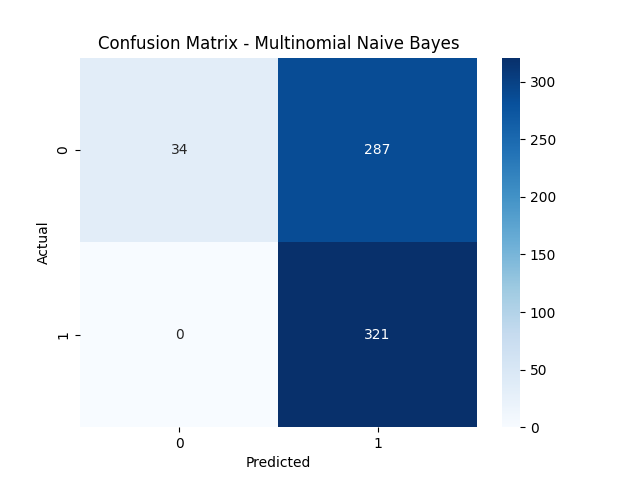
\includegraphics[width=0.6\textwidth,height=0.6\textheight, keepaspectratio]{figures/withoutgridsearch/NB.png}
  \caption{Confusion Matrix of Multinomial Naive Bayes without Grid Search}
  \label{CMofMNBwoGS}
\end{figure}

As shown in the confusion matrix of \textbf{Logistic Regression} at Figure \ref{CMofLRwoGS}, the model only misclassifies five fake news as real news and 12 real news as fake news. It yields an accuracy of approximately 0.97. It has a high recall for class 1 at 0.96. The f1-scores for both class 1 and 0 are 0.97.

\begin{figure}[ht]
\centering
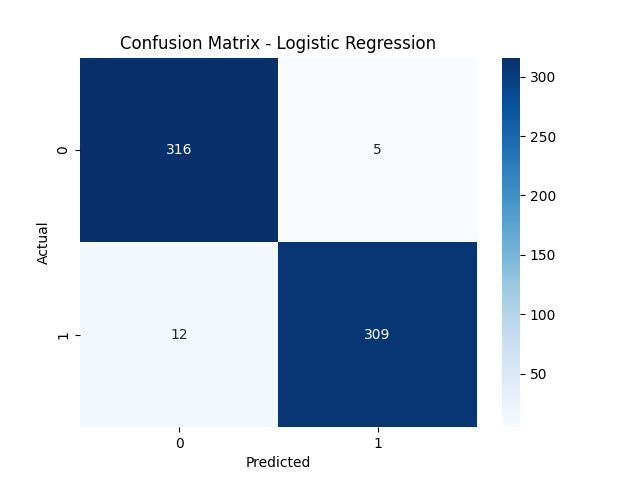
\includegraphics[width=0.6\textwidth,height=0.6\textheight, keepaspectratio]{figures/withoutgridsearch/LR.png}
  \caption{Confusion Matrix of Logistic Regression without Grid Search}
  \label{CMofLRwoGS}
\end{figure}

\clearpage

Figure \ref{CMofRFwoGS} depicts the confusion matrix of \textbf{Random Forest}. The model misclassifies 12 fake news and 20 real news. It yields an accuracy of approximately 0.95. It has a high recall for class 1 at 0.94. The f1-score of both classes is 0.95, showing balanced metrics.

\begin{figure}[ht]
\centering
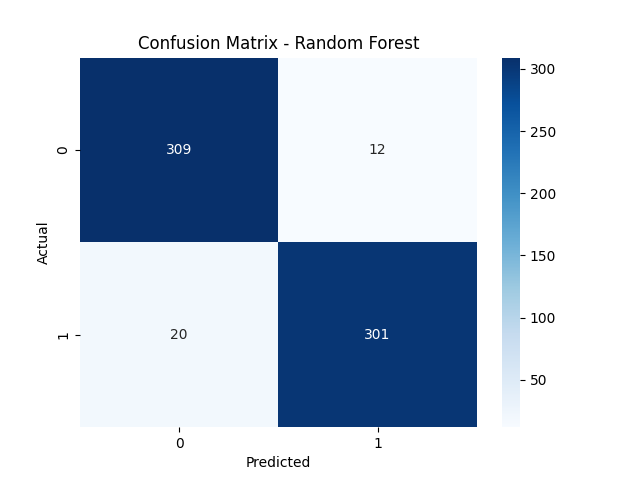
\includegraphics[width=0.6\textwidth,height=0.6\textheight, keepaspectratio]{figures/withoutgridsearch/RF.png}
  \caption{Confusion Matrix of Random Forest without Grid Search}
  \label{CMofRFwoGS}
\end{figure}

Based on Figure \ref{CMofSVCwoGS}, \textbf{SVC} misclassifies 99 fake news and 42 real news. Thus, it has an accuracy of approximately 0.78. It has a lower recall for class 0 at 0.69. The f1-score of classes 1 and 0 is 0.80 and 0.76, respectively. However, SVC has a slight imbalance in precision and recall for both classes.

\begin{figure}[ht]
\centering
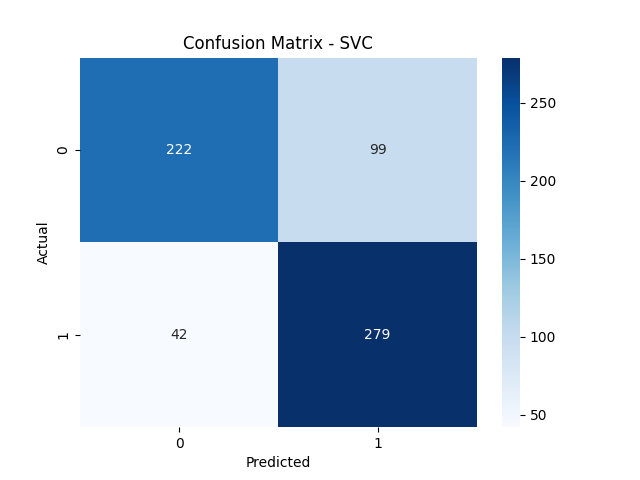
\includegraphics[width=0.6\textwidth,height=0.6\textheight, keepaspectratio]{figures/withoutgridsearch/SVC.png}
  \caption{Confusion Matrix of Support Vector Classifier without Grid Search}
  \label{CMofSVCwoGS}
\end{figure}

\clearpage

Our \textbf{Voting Classifier} misclassifies 11 fake news and 15 real news as shown in Figure \ref{CMofVCwoGS}. It has an accuracy of approximately 0.96. The recall of class 1 and 0 is 0.95 and 0.97, respectively. The f1-score of both class 1 and 0 is 0.96. Similar to Random Forest, both classes in this method also show balanced metrics.

\begin{figure}[ht]
\centering
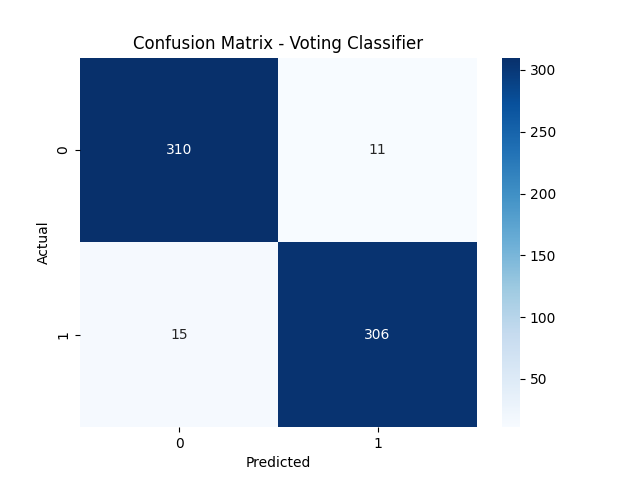
\includegraphics[width=0.6\textwidth,height=0.6\textheight, keepaspectratio]{figures/withoutgridsearch/VC.png}
  \caption{Confusion Matrix of Voting Classifier without Grid Search}
  \label{CMofVCwoGS}
\end{figure}

\clearpage

We summarize our results without using grid search in the Tables \ref{tab:classifier-metrics} and \ref{tab:voting-classifier-metrics}. As shown in Table \ref{tab:classifier-metrics}, Logistic Regression has the highest F1-Scores while Multinomial Naive Bayes has the lowest.

\begin{table}[ht]
\centering
\begin{tabular}{|l|ccc|ccc|}
\hline
& \multicolumn{3}{c|}{Multinomial Naive Bayes} & \multicolumn{3}{c|}{Logistic Regression} \\
\hline
& Precision & Recall & F1-Score & Precision & Recall & F1-Score \\
\hline
Fake & 1.00 & 0.11 & 0.19 & 0.96 & 0.98 & 0.97 \\
Not Fake & 0.53 & 1.00 & 0.69 & 0.98 & 0.96 & 0.97 \\
Accuracy & & & 0.55 & & & 0.97 \\
\hline
& \multicolumn{3}{c|}{Random Forest} & \multicolumn{3}{c|}{SVC} \\
\hline
& Precision & Recall & F1-Score & Precision & Recall & F1-Score \\
\hline
Fake & 0.94 & 0.96 & 0.95 & 0.84 & 0.69 & 0.76 \\
Not Fake & 0.96 & 0.94 & 0.95 & 0.74 & 0.87 & 0.80 \\
Accuracy & & & 0.95 & & & 0.78 \\
\hline
\end{tabular}
\caption{Performance Metrics for Classifiers without Grid Search}
\label{tab:classifier-metrics}
\end{table}

\begin{table}[ht]
\centering
\begin{tabular}{|l|ccc|}
\hline
& \multicolumn{3}{c|}{Voting Classifier} \\
\hline
& Precision & Recall & F1-Score \\
\hline
0 & 0.95 & 0.97 & 0.96 \\
1 & 0.97 & 0.95 & 0.96 \\
Accuracy & & & 0.96 \\
\hline
\end{tabular}
\caption{Performance Metrics for Voting Classifier without Grid Search}
\label{tab:voting-classifier-metrics}
\end{table}

\clearpage

\section{Classifiers with Grid Search}

Figure \ref{CMofMNBwGS} shows that \textbf{Multinomial Naive Bayes} with hyperparameter tuning misclassifies 42 fake news and four real news. It yields an accuracy of approximately 0.93. It has the lowest recall for class 0 at 0.87. However, this score is still relatively high. The minimum f1-score of both classes is 0.92 with the best feature as alpha=0.1. Hyperparameter tuning in Multinomial Naive Bayes has significantly improved balance between precision and recall for both classes.

\begin{figure}[ht]
\centering
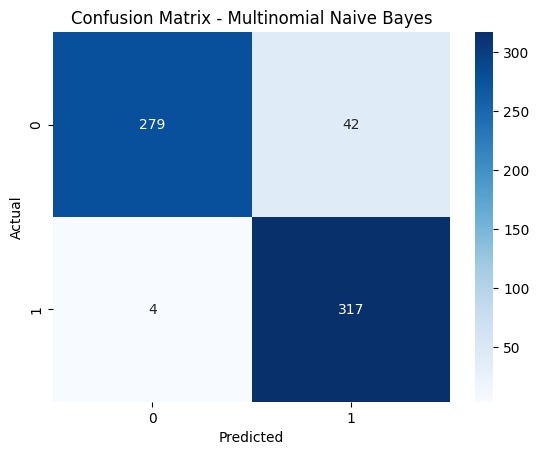
\includegraphics[width=0.5\textwidth,height=0.5\textheight, keepaspectratio]{figures/withgridsearch/NB.png}
  \caption{Confusion Matrix of Multinomial Naive Bayes with Grid Search}
  \label{CMofMNBwGS}
\end{figure}

\clearpage

\textbf{Logistic Regression}, on the other hand, misclassifies five fake news and 12 real news as shown in Figure \ref{CMofLRwGS}, which is still the same as before applying grid search. It yields an accuracy of approximately 0.97. It still has a high recall for class 1 of 0.96. Both classes have 0.97 f1-score. The best feature during hyperparameter tuning is max\_iter=2000.

\begin{figure}[ht]
\centering
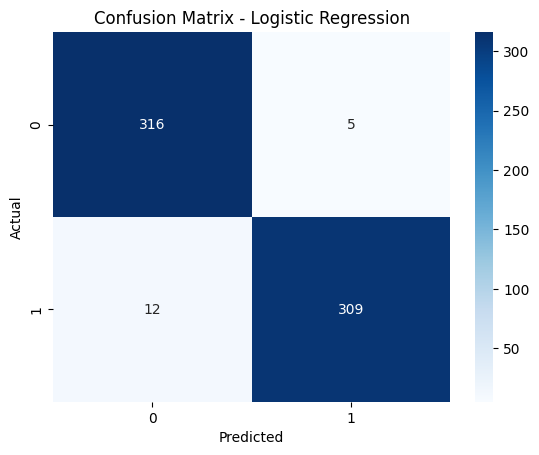
\includegraphics[width=0.5\textwidth,height=0.5\textheight, keepaspectratio]{figures/withgridsearch/LR.png}
  \caption{Confusion Matrix of Logistic Regression with Grid Search}
  \label{CMofLRwGS}
\end{figure}

\clearpage

Figure \ref{CMofRFwGS} shows that \textbf{Random Forest} misclassifies 22 fake news and 28 real news. Thus, it yields an accuracy of approximately 0.92. It has a high recall for class 1 at 0.91. Both classes have 0.92 f1-score. In hyperparameter tuning, its best features are max\_depth=20 and n\_estimators=50. But even with hyperparameter tuning, it provides the same balanced performance with minimal improvements.

\begin{figure}[ht]
\centering
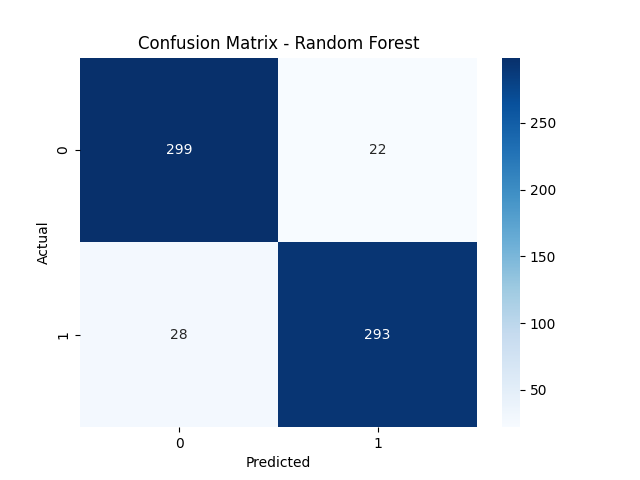
\includegraphics[width=0.58\textwidth,height=0.58\textheight, keepaspectratio]{figures/withgridsearch/RF.png}
  \caption{Confusion Matrix of Random Forest with Grid Search}
  \label{CMofRFwGS}
\end{figure}

\clearpage

For \textbf{SVC}, Figure \ref{CMofSVCwGS} shows that the model misclassifies five fake news and 14 real news with hyperparameter tuning. It yields an accuracy of approximately 0.97. It has a high recall for class 1 at 0.96. Both of the classes have a 0.97 f1-score. In tuning SVC, the best features are C=0.1 and kernel='linear'.

\begin{figure}[ht]
\centering
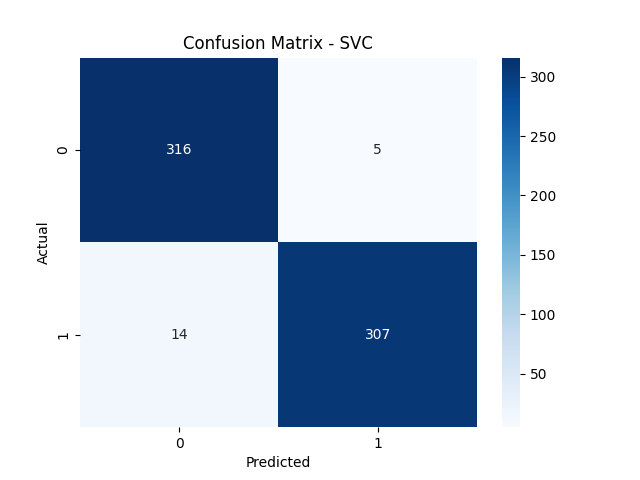
\includegraphics[width=0.6\textwidth,height=0.6\textheight, keepaspectratio]{figures/withgridsearch/SVC.png}
  \caption{Confusion Matrix of Support Vector Classifier with Grid Search}
  \label{CMofSVCwGS}
\end{figure}

Figure \ref{CMofVCwGS} shows that our \textbf{Voting Classifier} with hyperparameter tuning misclassifies five fake news and 13 real news. It yields an accuracy of approximately 0.97. It has a recall of 0.96 for class 1. Both classes have 0.97 f1-score. During tuning, the best feature is voting='soft'.

\begin{figure}[ht]
\centering
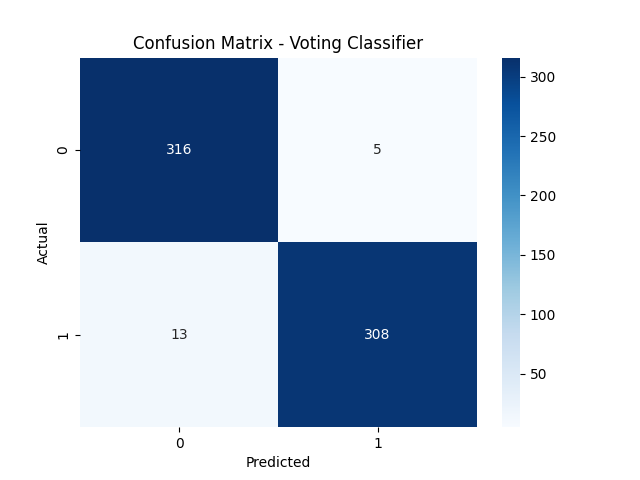
\includegraphics[width=0.6\textwidth,height=0.6\textheight, keepaspectratio]{figures/withgridsearch/VC.png}
  \caption{Confusion Matrix of Voting Classifier with Grid Search}
  \label{CMofVCwGS}
\end{figure}

\clearpage

We summarize our results by using grid search in the Tables \ref{tab:classifier-metrics-updated} and \ref{tab:voting-classifier-metrics-updated}. As shown in Table \ref{tab:classifier-metrics-updated}, both Logistic Regression and Support Vector Classifier has the highest F1-Scores while Random Forest has the lowest.

\begin{table}[ht]
\centering
\begin{tabular}{|l|ccc|ccc|}
\hline
& \multicolumn{3}{c|}{Multinomial Naive Bayes} & \multicolumn{3}{c|}{Logistic Regression} \\
\hline
& Precision & Recall & F1-Score & Precision & Recall & F1-Score \\
\hline
Fake & 0.99 & 0.87 & 0.92 & 0.96 & 0.98 & 0.97 \\
Not Fake & 0.88 & 0.99 & 0.93 & 0.98 & 0.96 & 0.97 \\
Accuracy & & & 0.93 & & & 0.97 \\
\hline
& \multicolumn{3}{c|}{Random Forest} & \multicolumn{3}{c|}{Support Vector Classifier} \\
\hline
& Precision & Recall & F1-Score & Precision & Recall & F1-Score \\
\hline
Fake & 0.91 & 0.93 & 0.92 & 0.96 & 0.98 & 0.97 \\
Not Fake & 0.93 & 0.91 & 0.92 & 0.98 & 0.96 & 0.97 \\
Accuracy & & & 0.92 & & & 0.97 \\
\hline
\end{tabular}
\caption{Performance Metrics for Classifiers with Grid Search}
\label{tab:classifier-metrics-updated}
\end{table}

\begin{table}[ht]
\centering
\begin{tabular}{|l|ccc|}
\hline
& \multicolumn{3}{c|}{Voting Classifier} \\
\hline
& Precision & Recall & F1-Score \\
\hline
Fake & 0.96 & 0.98 & 0.97 \\
Not Fake & 0.98 & 0.96 & 0.97 \\
Accuracy & & & 0.97 \\
\hline
\end{tabular}
\caption{Performance Metrics for Voting Classifier with Grid Search}
\label{tab:voting-classifier-metrics-updated}
\end{table}

\clearpage

\section{Preliminary Discussion}
The results before applying hyperparameter tuning reveal the ineffectiveness of Multinomial Naive Bayes, showing an accuracy of 0.55 and the lowest recall of 0.11 contrary to established literature. We hypothesize that this discrepancy is due to our Filipino corpus — previous studies train Multinomial Naive Bayes with an English corpus. In contrast, the effectiveness of Logistic Regression at 0.97 and Random Forest at 0.95 accuracy is apparent. However, we attempt to improve all of the classifiers with hyperparameter tuning via grid search. We find that hyperparameter tuning yields significant improvements on the lowest accuracy models but non-significant improvements on the rest of the models that already have high accuracy. Our results concur with previous studies, where Random Forest and Logistic Regression are also among the most accurate classifiers in fake news detection.

Among the machine learning models investigated, Logistic Regression exhibits consistently accurate performance before and after applying hyperparameter tuning. With our findings, we consider it as the primary candidate for future system deployment. However, the other models may serve the purposes of deployment better as computational efficiency and model size should be evaluated and considered when incorporating trained classifiers into a system. Currently, we have deployed the aforementioned Logistic Regression model that has achieved 97.4\% accuracy in a fully functional system (FaKe), available as a pre-release at \url{https://github.com/WhiteLicorice/Fake}. The repository also contains instructions for usage and installation. All resources used in this study are also available in the repository.

As an aside, we believe that it is difficult to score an accuracy greater than 0.97 due to our use of traditional machine learning models and our low-resource dataset. For future work, we will follow through with augmenting the dataset to possibly enhance results and further expand the domain of the corpus. Incorporation of more Filipino linguistic features (e.g. lexical, morphological, etc.) will be explored. Further experimentation with hyperparameter tuning may yield potential improvements.